\section{Evaluation}



\subsection{Stresstest zur Ressourcen- und Performance-Analyse}
Um den Ressourcenverbrauch und die Performance des Frameworks unter Mehrfachverbindungen zu analysieren,
wurde ein Stresstest durchgeführt.
Im Fokus standen dabei insbesondere die Ausführung von Animationen sowie die Berechnung der Vorwärts- und Rückwärtstransformationen während des Betriebs,
da das Funktionen sind die im realen Betrieb durchgehend aufgerufen werden.
Das Laden der Meshes wurde in diesem Test nicht berücksichtigt,
da es lediglich einmalig beim Start des Frameworks erfolgt.


\subsubsection{Testaufbau}
Der Stresstest wurde im Computerraum C.1.30 des Fachbereichs Informatik der Fachhochschule Dortmund durchgeführt.
Dabei kam ein Laptop der Marke HP (System B LT, siehe Tabelle \ref{tab:system_b_lt}) als Server zum Einsatz.
Als Clients wurden acht Workstations der Marke Dell (System C WS, siehe Tabelle \ref{tab:system_c_ws}) verwendet.
Für die Netzwerkkommunikation wurde ein Access Point der Marke TP-Link (System D AP, siehe Tabelle \ref{tab:system_d_ap}) eingesetzt.
Server und Clients waren über WLAN mit dem Access Point verbunden.


\vspace{1em}
\begin{figure}[H]
    \centering
    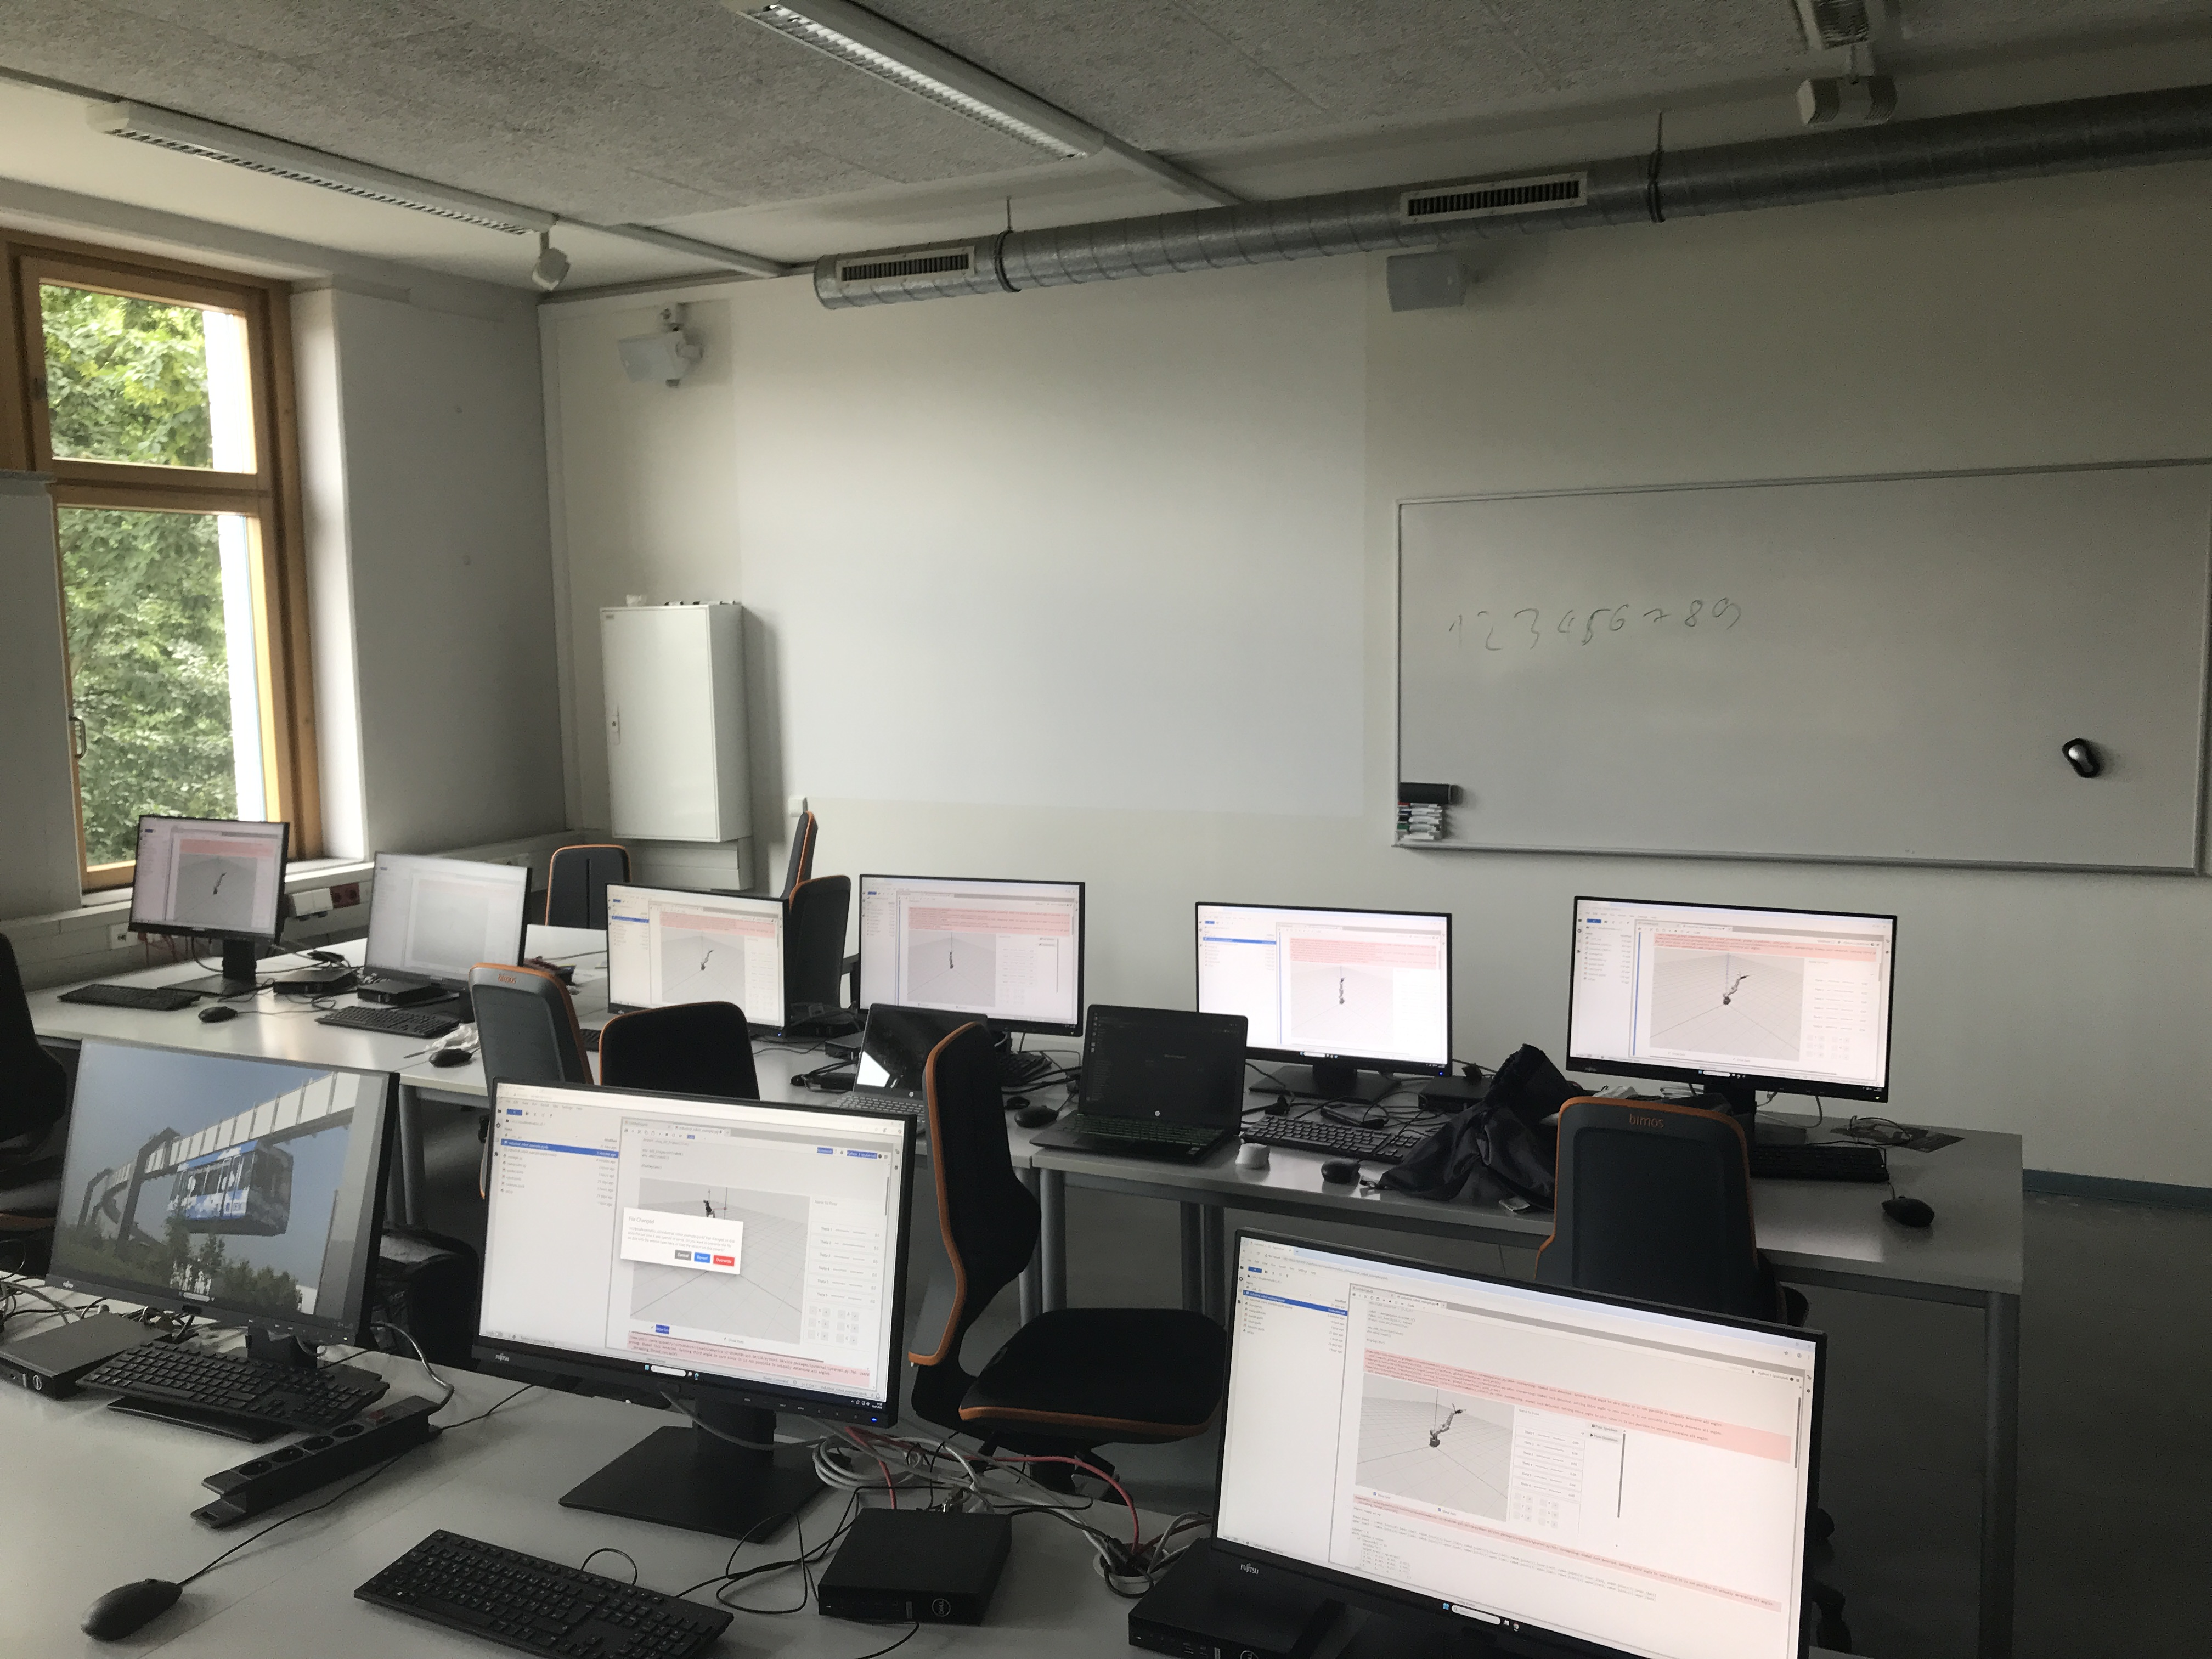
\includegraphics[width=0.8\textwidth]{images/aufbau.JPG}
    \caption{Testaufbau der Ressourcen- und Performance-Analyse}
    \label{fig:aufbau}
\end{figure}
\vspace{1em}


\subsubsection{Durchführung}
Auf dem System B LT wurden 8 unabhängige JupyterLab-Instanzen jeweils mit einem eigenen Kernel-Prozess gestartet.
Auf jedem der 8 Clients wurde ein Browser-Tab in Google Chrome geöffnet, um eine Verbindung zu jeweils einem dieser Kernel herzustellen.
Dadurch war jedem Kernel genau ein Client zugeordnet und umgekehrt. 
Auf jedem der Clients wurde eine Dauerschleife ausgeführt in der fortlaufend die Rückwärtstransformation berechnet und eine Animation durchgeführt wurde.
Die Rückwärtstransformation beinhaltet dabei die Berechnung der Vorwärtstransformation.
Zur Messung der Systemauslastung auf dem Server (System B LT) wurde über eine Dauer von 3 Minuten alle 5 Sekunden die Ausgabe des Kommandozeilenwerkzeugs top in eine Datei geschrieben.
Auf einem der Clients wurden während der Ausführung die Auslastungswerte des Taskmanagers mithilfe des Snipping Tools dokumentiert.
Anschließend wurde der gleiche Test erneut durchgeführt,
jedoch mit nur 4 Clients und 4 JupyterLab-Instanzen bzw. Kernel-Prozessen.

\subsubsection{Ergebnisse}
Die top-Ausgabe zeigt für 8 Instanzen eine durchschnittliche CPU-Auslastung von 98.8\% davon 92.33\% im User Space wo die JupyterLab-Instanzen ausgeführt worden sind.
Der Load Average lag bei 12.15.
Die gesamte RES-Speichernutzung der 8 JupyterLab-Instanzen lag im Durchschnitt bei 3483.22\,MiB
Für 4 Instancen lag eine durchschnittliche CPU-Auslastung von 98.9\% davon 69.57\% im User Space.
Der Load Average lad hier bei 8.07.
Die gesamte RES-Speichernutzung bei 1621.85\,MiB



\begin{table}[ht]
\centering
\begin{tabular}{|c|c|c|c|c|}
\hline
\textbf{Inst.} & \textbf{CPU Auslastung (\%)} & \textbf{User Space (\%)} & \textbf{Load Average} & \textbf{RES (MiB)} \\
\hline
8 & 98{,}8 & 92{,}3 & 12{,}15 & 3483{,}22 \\
4 & 98{,}9 & 69{,}6 & 8{,}07 & 1621{,}85 \\
\hline
\end{tabular}
\caption{Systemauslastung bei 4 und 8 JupyterLab-Instanzen}
\label{tab:jupyterlab}
\end{table}


Zusätzlich zur Systemauslastung wurde das Verhalten der Clients während des Tests beobachtet.
Trotz der hohen CPU-Last auf dem Server (System B LT) lief die Animation auf allen Clients durchgehend flüssig ab.
Auch die Berechnung der Rückwärtstransformationen zeigte keine spürbaren Verzögerungen im Ablauf.
Zwar wurden hierfür keine exakten Zeitmessungen durchgeführt,
jedoch ergaben sich augenscheinlich keine nennenswerten Beeinträchtigungen der Benutzererfahrung.

Der Taskmanager des Clients zeigte eine CPU Auslastung von 12\%, eine GPU Auslastung von 18\% und 7.2\,GB belegter RAM.


\subsubsection{Interpretation}
Die Messergebnisse verdeutlichen,
dass bereits bei 4 gleichzeitig verbundenen Clients eine nahezu vollständige Auslastung der CPU des Testsystems (System B LT) erreicht wurde.
Bei 8 Instanzen stieg die CPU-Auslastung im User Space von 69.6\% auf 92.3\%, was auf eine erhebliche Steigerung der Rechenlast durch die zusätzlichen JupyterLab-Instanzen hinweist.

Der Load Average überschritt in beiden Fällen deutlich die Anzahl verfügbarer logischer CPU-Kerne (vermutlich 4 Threads),
was bedeutet, dass viele Prozesse gleichzeitig auf CPU-Zeit warteten.
Besonders bei 8 Instanzen mit einem Load Average von 12.15 ist eine deutliche Systemüberlastung erkennbar.

Der Arbeitsspeicherverbrauch stieg bei 8 Instanzen auf mehr als das Doppelte im Vergleich zu 4 Instanzen.
Dies ist erwartbar, da jede Instanz Speicher benötigt, allerdings zeigt sich auch ein zusätzlicher Overhead pro Instanz.

Diese Ergebnisse zeigen, dass das verwendete Testsystem (System B LT) an seine Kapazitätsgrenzen gelangt.
Da es sich hierbei nicht um das geplante produktive System handelt,
können die Werte nicht unmittelbar auf die spätere Einsatzumgebung übertragen werden.
Sie zeigen jedoch, dass bei Mehrfachnutzung eine ausreichend leistungsfähige Serverhardware erforderlich ist.

Die Tatsache, dass die Animation auf den Clients dennoch Flüssig lief bestätigt, dass die Berechnungen für das
Rendering im Frontend durchgeführt werden und das Framework somit trotz überlastung eine stabile Nutzererfahrung ermöglicht.
Dies erklärt auch die leicht erhöhte GPU Auslastung auf dem Client.